\section{Additional \task Details}
\label{sec:task-details} 


\begin{figure*}[t]
  \centering
  \begin{subfigure}[t]{0.3\columnwidth}
    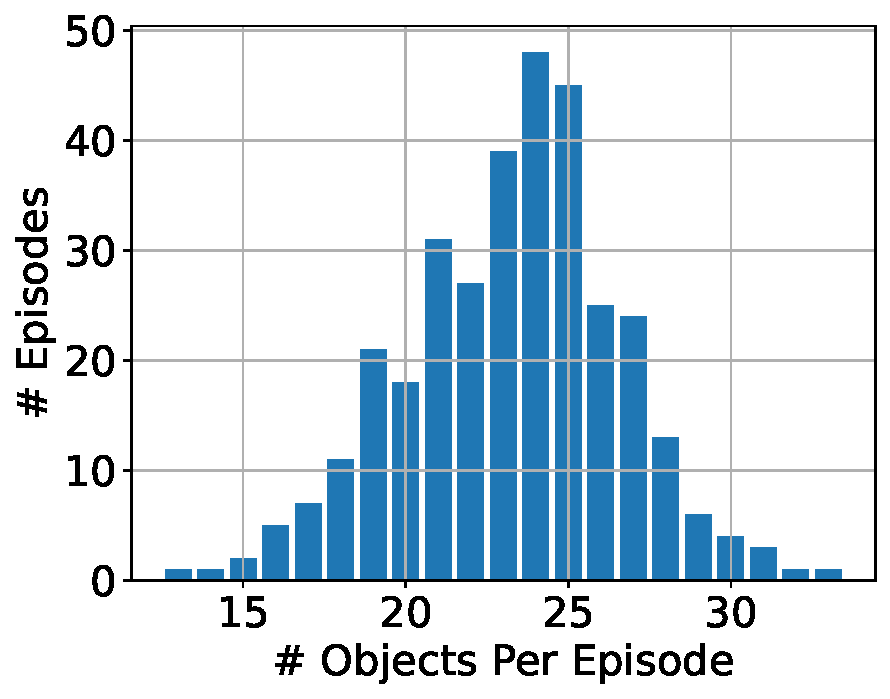
\includegraphics[width=\textwidth]{figures/results/data_dist_objPeps.pdf}
    \caption{\# Objects Per Episode}
  \end{subfigure}
  \begin{subfigure}[t]{0.3\columnwidth}
    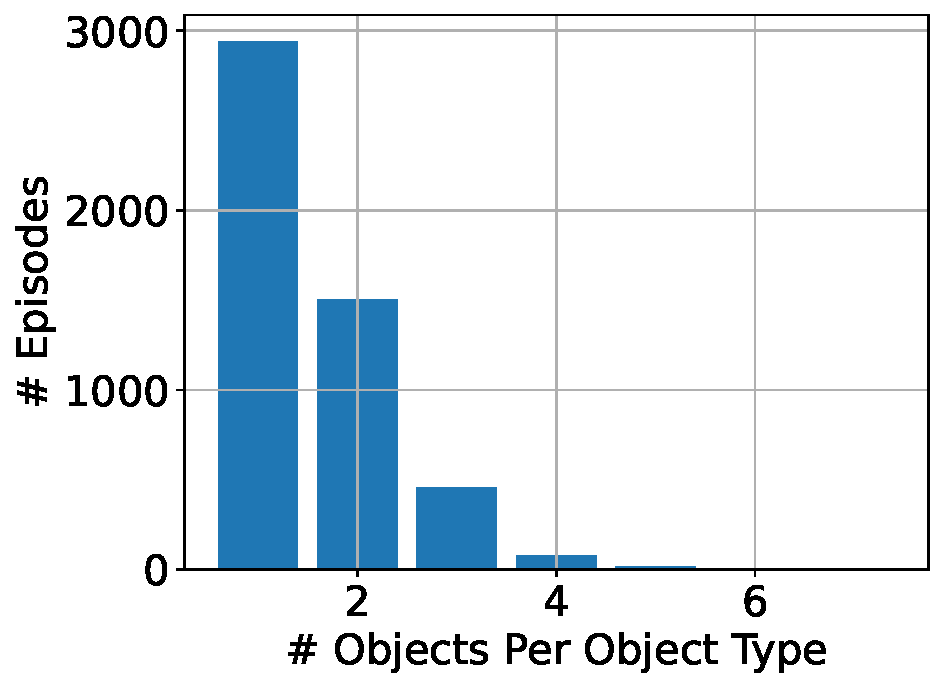
\includegraphics[width=\textwidth]{figures/results/data_dist_objPobjtype.pdf}
    \caption{\# Objects Per Object Type}
  \end{subfigure}
  \begin{subfigure}[t]{0.3\columnwidth}
    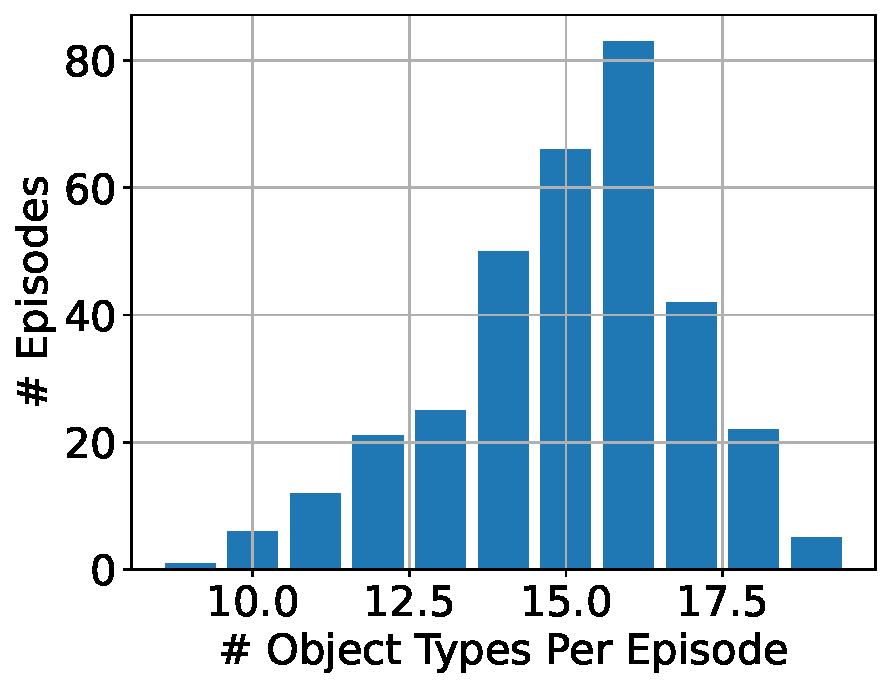
\includegraphics[width=\textwidth]{figures/results/data_dist_TypPeps.pdf}
    \caption{\# Object Types Per Episode}
  \end{subfigure}
  \caption{
    The distribution of the objects and object types in the data.
  }
  \label{fig:app-data-dist}
\end{figure*}


The \task is a small object navigation task. We use the same training (37) and validation (12) scenes as \cite{yenamandra2023homerobot}. The data is generated by randomly placing objects from the 20 object types, a subset of the YCB \cite{calli2015ycb} dataset, on random receptacles. The data is generated by sampling between 30 to 40 object instances and placing them on receptacles, and subsequent filtering of the objects that are not reachable by the agent. The filtering is done by placing the agent in front of the object and evaluating whether the agent can meet the success criteria. If the agent can meet the critera, we retain the object. Otherwise, we discard the object. The distribution of the objects and object types are in \Cref{fig:app-data-dist}.

The reward function is defined as follows:
\begin{itemize}[itemsep=2pt,topsep=0pt,parsep=0pt,partopsep=0pt,parsep=0pt,leftmargin=*]
    \item Change in geodesic distance to the closest object $r_d=-\Delta{d}$ where $d$ is the geodesic distance to the closest object. The closest object can change across the episode.
    \item Slack reward of $-0.001$.
    \item Succes reward of $2$.
\end{itemize}

The episode is considered a success if the agent selects the \textit{Stop} action while it is within 2 meters of an instance of the target type and has 10 pixels of this instance in the view.



